\documentclass{article}
\usepackage{graphicx}
\usepackage[
    colorlinks=true,        % Use colored links instead of boxes
    linkcolor=blue,         % Color for internal links
    urlcolor=blue,           % Color for URLs
    citecolor=green,        % Color for citations
    filecolor=magenta,      % Color for file links
    pdfborder={0 0 0}       % Remove border around links
]{hyperref}
\usepackage{ulem}
\let\oldhref\href
\renewcommand{\href}[2]{\uline{\oldhref{#1}{#2}}}

\usepackage{float} 

\title{COSC345 Assignment 1: Run It Twice}
\author{Run It Twice Team}
\date{\today}

\begin{document}

\maketitle

\section*{The Project: Run It Twice}
Our project aims to create a robust No Limit Holdem' (NLHE) poker training application designed for Windows terminal-based environments using C++. The app will offer a variety of game modes, including Training and Challenge modes, allowing users to practice against AI opponents of varying difficulty levels. It will feature educational resources, analytics, and feedback to help players improve their skills and track their progress.

\section*{Team Members}

\subsubsection*{Jess Tyrrell}
Jess is a passionate software developer with a keen interest in maths and poker. Jess will be responsible for the mathematical aspects of the project, including the AI players and game logic.

\subsubsection*{James Robiony-Rogers}
James brings significant experience in software development and project management. He has a strong background in object-oriented programming and writing clear, well-commented code. James will be responsible for the project management, enforcing conventional coding practices, and ensuring the project is delivered on time.

\subsubsection*{Corban Surtees}
Corban is a junior software developer with experience in C++, working with git, and interacting with command line interfaces. Corban will be responsible for developing the main architecture of the project and solving any issues with git.
\\ \\
Together, this team combines the skills necessary to deliver a high-quality, well-designed poker training application.

\section*{``Back to Basics" Approach}
To uphold our "Back to Basics" approach, our project will be written in C++ without external libraries. This ensures that we focus on fundamental programming principles and low-level coding techniques. We'll interact with our application solely through the terminal for user input and output, without any graphical user interface (GUI).
\\ \\
By narrowing the project scope, we aim to create a robust core application that performs its primary function effectively. However, we have also allowed for the possibility of expanding the project's features based on available resources and time. 

\section*{Project Development}
Run it Twice will be developed using the following tools and methodologies:

\begin{itemize}
    \item Agile Scrum methodology to manage the project in a flexible way.
    \item Object-oriented design allowing for the underlying code to be easily ported to any GUI.
    \item Visual Studio Code for our development environment.
    \item Discord group chat as our communication platform. You can join our Discord server by following this link: \href{https://discord.gg/jnGg3t9h7V}{Join our Discord server}.
    \item GitHub Project board for tracking issues, bugs, and the project's development.
    \item We have arranged two 2-hour meeting times every week dedicated to peer programming and project organization.
\end{itemize}

\section*{Project Schedule}

During requirements elicitation we created user stories and identified key milestones in the project. These were represented in the Gantt Chart in Figure \ref{fig:project_schedule}. 

\begin{figure}[H]
    \centering
    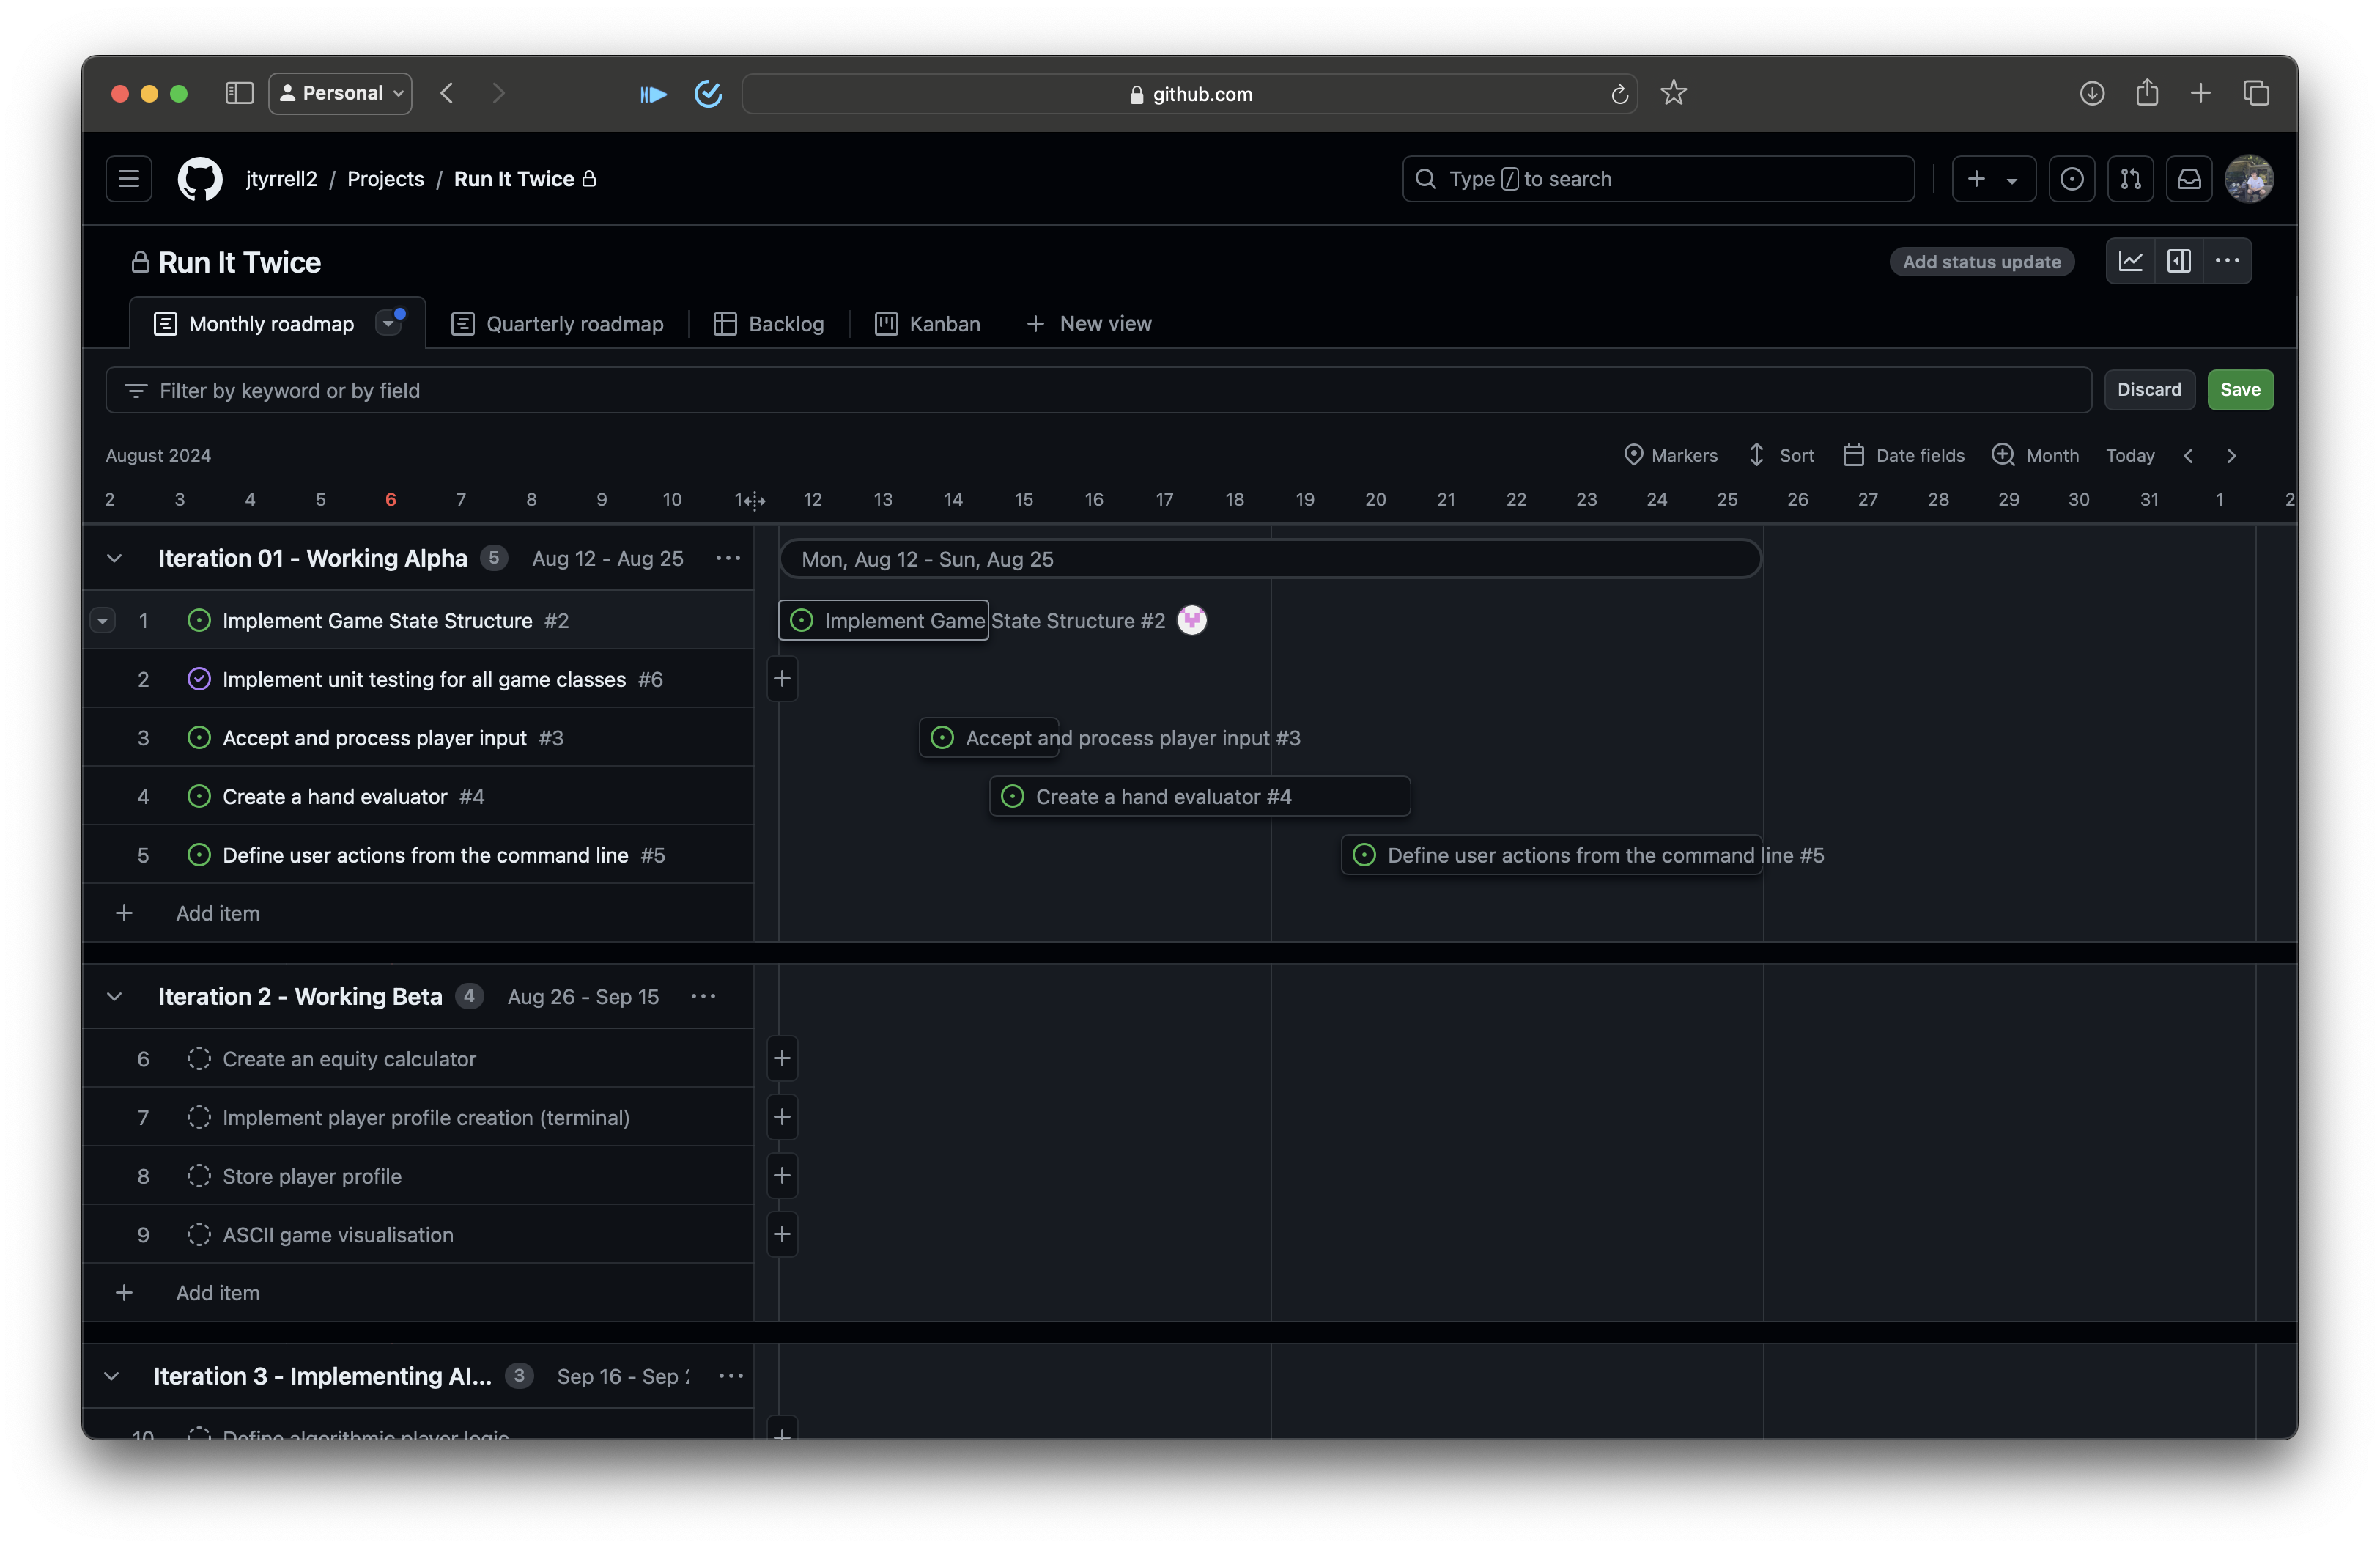
\includegraphics[width=\textwidth]{ProjectSchedule.png}
    \caption{Project Gantt Chart}
    \label{fig:project_schedule}
\end{figure}


\section*{Similar Applications}

\subsection*{Poker Trainer - \href{https://pokertrainer.se/}{https://pokertrainer.se/}}
Poker Trainer offers a dynamic, exercise-based training system with options available to players of variable skill level. Users are able to select particular areas of their game they want to master. 
\\ \\
Inspired to produce a competitive product, our project will also have difficulty settings and AI players that have tendencies to make different mistakes. This will allow our application to give feedback to the user by identifying which AI players a user performs better against.

\subsection*{Run It Once - \href{https://www.runitonce.com/}{https://www.runitonce.com/}}
 Run it Once is a poker website featuring videos from professional players and a robust library of hand analyses. It provides these resources for a number of different types of poker, while our application will be exclusively for NLHE.

\section*{Customer Interest}
Poker remains one of the most popular card games globally, with millions of players looking for ways to enhance their skills. As more people engage with poker, the demand for effective training tools has also risen. Players are now seeking ways to enhance their strategies and improve their game-play, both at the physical and virtual felt.
\\ \\
Existing applications such as `Poker Trainer' and `Run It Once' have seen significant success, highlighting a robust market for our application.
\\ \\
While most modern applications prioritize graphical user interfaces, our command-line-based approach offers several unique advantages that align with our "Back to Basics" philosophy. A command-line interface (CLI)  eliminates distractions and forces users to focus solely on the core aspects of game-play and strategy, without the potential clutter or visual noise of a GUI. This minimalist approach encourages a deeper understanding of the game mechanics, as users must interact with the app more intentionally.
\\ \\
Furthermore, many existing poker training tools depend on web-based platforms that require a continuous internet connection. By utilising a CLI, our application bypasses this limitation, allowing users to train offline without the need for constant connectivity.
\\ \\
We strongly believe that our application will be useful to anyone who plays poker to learn and fine-tune poker fundamentals. Utilising AI, we will deliver a training environment that replicates playing at a real table. By tracking detailed statistics, we will be able to precisely gauge when users have achieved their desired level of proficiency.
\end{document}
